\documentclass{article}
\usepackage{amsmath}
\usepackage{amssymb}
\usepackage{graphicx}
\usepackage{hyperref}
\usepackage[version=4]{mhchem}


\begin{document}
In \(\triangle A B C, C D\) is altitude and \(C M\) is the median. What is the measure of \(\angle C\) if \(C D\) and \(C M\) trisect \(\angle C\) ?

Solution: \(90^{\circ}\).\\
Draw the perpendicular line \(M K\) and \(M K \perp B C\) at \(K\).\\
\centering
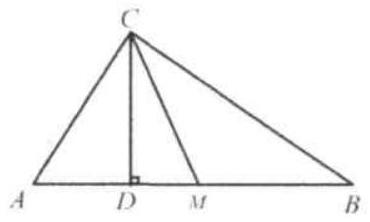
\includegraphics[width=\textwidth]{images/081(3).jpg}

Since \(\angle A C D=\angle D C M=\angle M C B, \triangle A C D \cong \triangle D C M \cong\) \(\triangle K C M\).\\
Thus \(A D=D M=K M\).\\
Since \(C M\) is the median, \(M B=M A=2 D M=2 K M\).\\
We then know that in right triangle \(B K M, \angle B=30^{\circ}\).\\
\centering
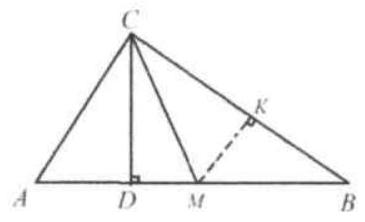
\includegraphics[width=\textwidth]{images/081(1).jpg}

So in right triangle \(B C D, \angle B C D=60^{\circ}\).\\
Then \(\angle A C D=\angle D C M=\angle M C B=30^{\circ}\) and \(\angle A C B=3 \times 30^{\circ}=90^{\circ}\).


\end{document}
